
{\setbeamercolor{background canvas}{bg=black}
	\begin{frame}[plain]
	\vfill
	\begin{columns}
		\column{.25\textwidth}
		\color{tumwhite}
		
		\Huge
		Gated Recurrence
		
		\column{.75\textwidth}
		\raggedleft
		\tikzstyle{rec} = [draw=white, fill=black, rounded corners, inner sep=2em]
		\begin{tikzpicture}[node distance=2em]
			\node[rec](rec){};
			\draw[-stealth, white, very thick] ($ (rec)+(0,5em) $) -- (rec) node[at start, above]{$\V{x}_t$};
			\draw[-stealth, white, very thick] (rec) -- ($ (rec)+(0,-5em) $) node[at end, below]{$\V{h}_t$};
			
			\draw[-stealth, white, very thick] (rec.south) to[in=270, out=250, looseness=2] ($ (rec.west)+(-1.5em,0) $) to[in=110, out=90, looseness=2] (rec.north) node[at start, left, xshift=-4em]{$\V{h}_{t-1}$};
			
			\node[rec, right=3em of rec](unrolled0){};
			\draw[-stealth, white, very thick] ($ (unrolled0)+(0,5em) $) -- (unrolled0) node[at start, above]{$\V{x}_1$};
			\draw[-stealth, white, very thick] (unrolled0) -- ($ (unrolled0)+(0,-5em) $) node[at end, below]{$\V{h}_1$};;
			
			\coordinate(sep) at ($ (rec)!0.5!(unrolled0) $);
			
			\draw[dotted, thick] ($ (sep)+(0,-5em) $) -- ($ (sep)+(0,5em) $);

			\node[rec, right=of unrolled0](unrolled1){};
			\draw[-stealth, white, very thick] ($ (unrolled1)+(0,5em) $) -- (unrolled1) node[at start, above]{$\V{x}_2$};
			\draw[-stealth, white, very thick] (unrolled1) -- ($ (unrolled1)+(0,-5em) $) node[at end, below]{$\V{h}_2$};
			
			\node[rec, right=of unrolled1](unrolled2){};
			\draw[-stealth, white, very thick] ($ (unrolled2)+(0,5em) $) -- (unrolled2) node[at start, above]{$\V{x}_3$};
			\draw[-stealth, white, very thick] (unrolled2) -- ($ (unrolled2)+(0,-5em) $) node[at end, below]{$\V{h}_3$};;
			
			\node[rec, right=of unrolled2](unrolled3){};
			\draw[-stealth, white, very thick] ($ (unrolled3)+(0,5em) $) -- (unrolled3) node[at start, above]{$\V{x}_4$};
			\draw[-stealth, white, very thick] (unrolled3) -- ($ (unrolled3)+(0,-5em) $) node[at end, below]{$\V{h}_4$};
			
			\draw[-stealth, white, very thick] (unrolled0) -- (unrolled1) node[near end, above]{$\V{h}_1$};
			\draw[-stealth, white, very thick] (unrolled1) -- (unrolled2) node[near end, above]{$\V{h}_2$};
			\draw[-stealth, white, very thick] (unrolled2) -- (unrolled3) node[near end, above]{$\V{h}_3$};
			
			
		\end{tikzpicture}
		
	\end{columns}
	\vfill
\end{frame}
}

\newcommand{\gates}[6]{
	\tikzstyle{gate} = [inner sep=0em, draw, rounded corners, minimum width=1.5em, minimum height=1.5em]
	\begin{tikzpicture}[xscale=0.75, yscale=-0.66]
		\node[gate,#2](i) at (0,0){$\V{i}_{#1}$};
		\node[gate,#3](f) at (0,1){$\V{f}_{#1}$};
		\node[gate,#4](g) at (1,0){$\V{g}_{#1}$};
		\node[gate,#5](o) at (1,1){$\V{o}_{#1}$};
		\node[gate,#6](c) at (0.5,2){$\V{c}_{#1}$};
		
		\node[font=\tiny, inner sep=0, minimum width=0, minimum height=0, rounded corners=0](thetai) at (i.south east){$\Mweight_i$};
		\node[font=\tiny, inner sep=0, minimum width=0, minimum height=0, rounded corners=0](thetai) at (f.south east){$\Mweight_f$};
		\node[font=\tiny, inner sep=0, minimum width=0, minimum height=0, rounded corners=0](thetai) at (g.south east){$\Mweight_g$};
		\node[font=\tiny, inner sep=0, minimum width=0, minimum height=0, rounded corners=0](thetai) at (o.south east){$\Mweight_o$};
	\end{tikzpicture}
}

\begin{frame}

%1 gates
%2 input gate
%3 modulation gate
%4 forget gate
%5 output gate
%6 cell state
%7 output

\frametitle{Long Short Term Memory (LSTM) Recurrent Network}
\tikzstyle{focused} = [fill=tumbluedark, text=white, draw, rounded corners, thin]
\tikzstyle{unfocused} = [fill=white, draw, rounded corners, thin]
\tikzstyle{background} = [fill=white, draw, rounded corners, thin, opacity=0.2]

\tikzstyle{rec} = [draw=tumbluedark, fill=none, rounded corners, inner sep=0em, minimum width=5em, minimum height=6em]
\tikzstyle{conn} = [-stealth, tumbluedark, very thick]

\begin{columns}
	
\column{.5\textwidth}
	
\begin{tikzpicture}[node distance=3em]

\node[rec, right=3em of rec, background](unrolled0){
	\only<1-5,7->{\gates{1}{unfocused}{unfocused}{unfocused}{unfocused}{unfocused}}
	\only<6>{\gates{1}{unfocused}{unfocused}{unfocused}{unfocused}{focused}}
};
\node[above=of unrolled0, background](x0){$\V{x}_1$};
\draw[conn, background] (x0) -- (unrolled0);
\draw[conn, background] (unrolled0) -- ($ (unrolled0)+(0,-5em) $);
\node[below=of unrolled0, background](h0){$\V{h}_1$};

\node[rec, right=of unrolled0](unrolled1){%i f g o c
	\only<1>{\gates{2}{background}{background}{background}{background}{unfocused}}%
	\only<2>{\gates{2}{focused}{unfocused}{unfocused}{unfocused}{unfocused}}%
	\only<3>{\gates{2}{unfocused}{unfocused}{focused}{unfocused}{unfocused}}%
	\only<4>{\gates{2}{unfocused}{focused}{unfocused}{unfocused}{unfocused}}%
	\only<5>{\gates{2}{unfocused}{unfocused}{unfocused}{focused}{unfocused}}%
	\only<6>{\gates{2}{focused}{focused}{focused}{unfocused}{focused}}%
	\only<7>{\gates{2}{unfocused}{unfocused}{unfocused}{focused}{focused}}%
};
\visible<2-5>{\node[above=of unrolled1, focused](x1){$\V{x}_2$};}
\visible<1,6->{\node[above=of unrolled1, unfocused](x1){$\V{x}_2$};}
\draw[conn] (x1) -- (unrolled1);
\draw[conn] (unrolled1) -- ($ (unrolled1)+(0,-5em) $);

\visible<7>{\node[below=of unrolled1, focused](h0){$\V{h}_2$};}
\visible<1-6>{\node[below=of unrolled1, unfocused](h0){$\V{h}_2$};}
%													  i f g o c
%\phantom{
%	\node[rec, right=of unrolled1](unrolled2){\gates{3}{unfocused}{unfocused}{unfocused}{unfocused}{unfocused}};
%	\draw[conn] ($ (unrolled2)+(0,5em) $) -- (unrolled2) node[at start, above]{$\V{x}_3$};
%	\draw[conn] (unrolled2) -- ($ (unrolled2)+(0,-5em) $) node[at end, below]{$\V{h}_3$};;
%}
\draw[conn] (unrolled0) -- (unrolled1);
\visible<1,5->{
	\node[unfocused, yshift=1em] at ($ (unrolled0)!0.5!(unrolled1) $){$\V{h}_1$};
}
\visible<2-5>{
	\node[focused, yshift=1em] at ($ (unrolled0)!0.5!(unrolled1) $){$\V{h}_1$};
}
\visible<1-5,7->{
	\node[unfocused, yshift=-1em] at ($ (unrolled0)!0.5!(unrolled1) $){$\V{c}_1$};
}
\visible<6>{
	\node[focused, yshift=-1em] at ($ (unrolled0)!0.5!(unrolled1) $){$\V{c}_1$};
}
%\visible<2-4>{
%	\draw[conn] (unrolled0) -- (unrolled1) node[midway, above, focused]{$\V{h}_1$} node[midway, below, focused]{$\V{c}_1$};
%}

%\visible<1-6>{\draw[conn] (unrolled1) -- (unrolled2) node[midway, above, unfocused]{$\V{h}_2$};}
%\visible<7>{\draw[conn] (unrolled1) -- (unrolled2) node[midway, above, focused]{$\V{h}_2$};}


\end{tikzpicture}

\column{.5\textwidth}

Long Short-Term Memory Neural Network (LSTM):
\begin{equation*}
	\V{h}_t, \V{c}_t \leftarrow \V{x}_t ,\V{h}_{t-1}, \V{c}_{t-1}
\end{equation*}
controlled by internal Gates:

\visible<2->{$\V{i_t} = \sigma\left(\V{x}_t\Mweight_{xi} + \V{h}_{t-1}\Mweight_{hi}\right)$}
\visible<3->{$\V{g_t} = \tanh\left(\V{x}_t\Mweight_{xg} + \V{h}_{t-1}\Mweight_{hg}\right)$}
\visible<4->{$\V{f_t} = \sigma\left(\V{x}_t\Mweight_{xf} + \V{h}_{t-1}\Mweight_{hf}\right)$}
\visible<5->{$\V{o_t} = \sigma\left(\V{x}_t\Mweight_{xo} + \V{h}_{t-1}\Mweight_{ho}\right)$}
\vspace{1em}

\visible<6->{$\V{c_t} = \V{f}_t*\V{c}_{t-1} + \V{i}_t \odot \V{g}_t$}

\visible<7->{$\V{h_t} = \V{o}_t \odot \tanh(\V{c_t})$}

\end{columns}

\end{frame}

%
%\begin{frame}<presentation:3>
%\frametitle{Employ ConvRNNs for Vegetation Land Cover Classification directly}
%%	\input{images/seqencnetwork.tikz}
%%	\figseqencnetwork
%\input{images/network.tikz}
%%	
%%	\input{images/lstm.tikz}
%%	\lstmanimtwo
%\end{frame}


\begin{frame}

\begin{tikzpicture}
%
%	\frametitle{Example}
%		
\def\i{20}
\def\root{images/rnn_examples/8}


\begin{groupplot}[
group style = {
	group size = 1 by 7,
	xlabels at=edge bottom,
	xticklabels at=edge bottom,
	vertical sep=0pt,
},
width=\textwidth,
%		hide axis,
enlargelimits=.1,
height=2.5cm,
%		ymin=0, ymax=1.4,
no marks,
]
\nextgroupplot[draw opacity=.8, smooth=0.01, thin]
\addplot[b11color, mark=*,mark size=.5pt] table [x=t, y=B11, col sep=comma, forget plot] {\root/x.csv};
\addplot[b12color, mark=*,mark size=.5pt] table [x=t, y=B12, col sep=comma] {\root/x.csv};

\addplot[b5color, mark=*,mark size=.5pt] table [x=t, y=B5, col sep=comma, forget plot] {\root/x.csv};
\addplot[b6color, mark=*,mark size=.5pt] table [x=t, y=B6, col sep=comma, forget plot] {\root/x.csv};
\addplot[b7color, mark=*,mark size=.5pt] table [x=t, y=B7, col sep=comma, forget plot] {\root/x.csv};
\addplot[b8color, mark=*,mark size=.5pt] table [x=t, y=B8, col sep=comma, forget plot] {\root/x.csv};
\addplot[b8Acolor, mark=*,mark size=.5pt] table [x=t, y=B8A, col sep=comma] {\root/x.csv};

\addplot[b2color, mark=*,mark size=.5pt] table [x=t, y=B2, col sep=comma, forget plot] {\root/x.csv};
\addplot[b3color, mark=*,mark size=.5pt] table [x=t, y=B3, col sep=comma, forget plot] {\root/x.csv};
\addplot[b4color, mark=*,mark size=.5pt] table [x=t, y=B4, col sep=comma] {\root/x.csv};

\nextgroupplot[cycle list name=featurecolorlist, draw opacity=.8, smooth=0.01, thin, ylabel=$\V{i}$]
\foreach \i in {0,1,...,31}{
	\addplot table [x=t, y=\i, col sep=comma] {\root/i.csv};
}
\nextgroupplot[cycle list name=featurecolorlist, draw opacity=.8, smooth=0.01, thin, ylabel=$\V{f}$]
\foreach \i in {0,1,...,31}{
	\addplot table [x=t, y=\i, col sep=comma] {\root/f.csv};
}
\nextgroupplot[cycle list name=featurecolorlist, draw opacity=.8, smooth=0.01, thin, ylabel=$\V{g}$]
\foreach \i in {0,1,...,31}{
	\addplot table [x=t, y=\i, col sep=comma] {\root/g.csv};
}
\nextgroupplot[cycle list name=featurecolorlist, draw opacity=.8, smooth=0.01, thin, ylabel=$\V{o}$]
\foreach \i in {0,1,...,31}{
	\addplot table [x=t, y=\i, col sep=comma] {\root/o.csv};
}
\nextgroupplot[cycle list name=featurecolorlist, draw opacity=.8, smooth=0.01, thin, ylabel=$\V{h}$]
\foreach \i in {0,1,...,31}{
	\addplot table [x=t, y=\i, col sep=comma] {\root/h.csv};
}
\nextgroupplot[cycle list name=featurecolorlist, draw opacity=.8, smooth=0.01, thin, ylabel=$\V{c}$]
\foreach \i in {0,1,...,31}{
	\addplot table [x=t, y=\i, col sep=comma] {\root/c.csv};
}

\end{groupplot}

\end{tikzpicture}
\end{frame}

\begin{frame}
\begin{tikzpicture}
%
%	\frametitle{Example}
%		
\def\i{20}
\def\root{images/rnn_examples/5}


\begin{groupplot}[
group style = {
group size = 1 by 7,
xlabels at=edge bottom,
xticklabels at=edge bottom,
vertical sep=0pt,
},
width=\textwidth,
%		hide axis,
enlargelimits=.1,
height=2.5cm,
%		ymin=0, ymax=1.4,
no marks,
]
\nextgroupplot[draw opacity=.8, smooth=0.01, thin]
\addplot[b11color, mark=*,mark size=.5pt] table [x=t, y=B11, col sep=comma, forget plot] {\root/x.csv};
\addplot[b12color, mark=*,mark size=.5pt] table [x=t, y=B12, col sep=comma] {\root/x.csv};

\addplot[b5color, mark=*,mark size=.5pt] table [x=t, y=B5, col sep=comma, forget plot] {\root/x.csv};
\addplot[b6color, mark=*,mark size=.5pt] table [x=t, y=B6, col sep=comma, forget plot] {\root/x.csv};
\addplot[b7color, mark=*,mark size=.5pt] table [x=t, y=B7, col sep=comma, forget plot] {\root/x.csv};
\addplot[b8color, mark=*,mark size=.5pt] table [x=t, y=B8, col sep=comma, forget plot] {\root/x.csv};
\addplot[b8Acolor, mark=*,mark size=.5pt] table [x=t, y=B8A, col sep=comma] {\root/x.csv};

\addplot[b2color, mark=*,mark size=.5pt] table [x=t, y=B2, col sep=comma, forget plot] {\root/x.csv};
\addplot[b3color, mark=*,mark size=.5pt] table [x=t, y=B3, col sep=comma, forget plot] {\root/x.csv};
\addplot[b4color, mark=*,mark size=.5pt] table [x=t, y=B4, col sep=comma] {\root/x.csv};

\nextgroupplot[cycle list name=featurecolorlist, draw opacity=.1, smooth=0.01, thin, ylabel=$\V{i}$]

\addplot table [x=t,  y=0, col sep=comma] {\root/i.csv};
\addplot table [x=t,  y=1, col sep=comma] {\root/i.csv};
\addplot table [x=t,  y=2, col sep=comma] {\root/i.csv};
\addplot table [x=t,  y=3, col sep=comma] {\root/i.csv};
\addplot table [x=t,  y=4, col sep=comma] {\root/i.csv};
\addplot table [x=t,  y=5, col sep=comma] {\root/i.csv};
\addplot table [x=t,  y=6, col sep=comma] {\root/i.csv};
\addplot table [x=t,  y=7, col sep=comma] {\root/i.csv};
\addplot table [x=t,  y=8, col sep=comma] {\root/i.csv};
\addplot table [x=t,  y=9, col sep=comma] {\root/i.csv};
\addplot table [x=t, y=10, col sep=comma] {\root/i.csv};
\addplot table [x=t, y=11, col sep=comma] {\root/i.csv};
\addplot table [x=t, y=12, col sep=comma] {\root/i.csv};
\addplot table [x=t, y=13, col sep=comma] {\root/i.csv};
\addplot table [x=t, y=14, col sep=comma] {\root/i.csv};
\addplot table [x=t, y=15, col sep=comma] {\root/i.csv};
\addplot table [x=t, y=16, col sep=comma] {\root/i.csv};
\addplot table [x=t, y=17, col sep=comma] {\root/i.csv};
\addplot table [x=t, y=18, col sep=comma] {\root/i.csv};
\addplot table [x=t, y=19, col sep=comma] {\root/i.csv};
\addplot table [x=t, y=20, col sep=comma] {\root/i.csv};
\addplot table [x=t, y=21, col sep=comma] {\root/i.csv};
\addplot table [x=t, y=22, col sep=comma] {\root/i.csv};
\addplot table [x=t, y=23, col sep=comma] {\root/i.csv};
\addplot table [x=t, y=24, col sep=comma] {\root/i.csv};
\addplot table [x=t, y=25, col sep=comma] {\root/i.csv};
\addplot table [x=t, y=26, col sep=comma] {\root/i.csv};
\addplot table [x=t, y=27, col sep=comma] {\root/i.csv};
\addplot table [x=t, y=28, col sep=comma] {\root/i.csv};
\addplot table [x=t, y=29, col sep=comma] {\root/i.csv};
\addplot[draw opacity=1] table [x=t, y=30, col sep=comma] {\root/i.csv};
\addplot table [x=t, y=31, col sep=comma] {\root/i.csv};

\nextgroupplot[cycle list name=featurecolorlist, draw opacity=.2, smooth=0.01, thin, ylabel=$\V{f}$]

\addplot table [x=t,  y=0, col sep=comma] {\root/f.csv};
\addplot table [x=t,  y=1, col sep=comma] {\root/f.csv};
\addplot table [x=t,  y=2, col sep=comma] {\root/f.csv};
\addplot table [x=t,  y=3, col sep=comma] {\root/f.csv};
\addplot table [x=t,  y=4, col sep=comma] {\root/f.csv};
\addplot table [x=t,  y=5, col sep=comma] {\root/f.csv};
\addplot table [x=t,  y=6, col sep=comma] {\root/f.csv};
\addplot table [x=t,  y=7, col sep=comma] {\root/f.csv};
\addplot table [x=t,  y=8, col sep=comma] {\root/f.csv};
\addplot table [x=t,  y=9, col sep=comma] {\root/f.csv};
\addplot table [x=t, y=10, col sep=comma] {\root/f.csv};
\addplot table [x=t, y=11, col sep=comma] {\root/f.csv};
\addplot table [x=t, y=12, col sep=comma] {\root/f.csv};
\addplot table [x=t, y=13, col sep=comma] {\root/f.csv};
\addplot table [x=t, y=14, col sep=comma] {\root/f.csv};
\addplot table [x=t, y=15, col sep=comma] {\root/f.csv};
\addplot table [x=t, y=16, col sep=comma] {\root/f.csv};
\addplot table [x=t, y=17, col sep=comma] {\root/f.csv};
\addplot table [x=t, y=18, col sep=comma] {\root/f.csv};
\addplot table [x=t, y=19, col sep=comma] {\root/f.csv};
\addplot table [x=t, y=20, col sep=comma] {\root/f.csv};
\addplot table [x=t, y=21, col sep=comma] {\root/f.csv};
\addplot table [x=t, y=22, col sep=comma] {\root/f.csv};
\addplot table [x=t, y=23, col sep=comma] {\root/f.csv};
\addplot table [x=t, y=24, col sep=comma] {\root/f.csv};
\addplot table [x=t, y=25, col sep=comma] {\root/f.csv};
\addplot table [x=t, y=26, col sep=comma] {\root/f.csv};
\addplot table [x=t, y=27, col sep=comma] {\root/f.csv};
\addplot table [x=t, y=28, col sep=comma] {\root/f.csv};
\addplot table [x=t, y=29, col sep=comma] {\root/f.csv};
\addplot[draw opacity=1] table [x=t, y=30, col sep=comma] {\root/f.csv};
\addplot table [x=t, y=31, col sep=comma] {\root/f.csv};

\nextgroupplot[cycle list name=featurecolorlist, draw opacity=.2, smooth=0.01, thin, ylabel=$\V{g}$]

\addplot table [x=t,  y=0, col sep=comma] {\root/g.csv};
\addplot table [x=t,  y=1, col sep=comma] {\root/g.csv};
\addplot table [x=t,  y=2, col sep=comma] {\root/g.csv};
\addplot table [x=t,  y=3, col sep=comma] {\root/g.csv};
\addplot table [x=t,  y=4, col sep=comma] {\root/g.csv};
\addplot table [x=t,  y=5, col sep=comma] {\root/g.csv};
\addplot table [x=t,  y=6, col sep=comma] {\root/g.csv};
\addplot table [x=t,  y=7, col sep=comma] {\root/g.csv};
\addplot table [x=t,  y=8, col sep=comma] {\root/g.csv};
\addplot table [x=t,  y=9, col sep=comma] {\root/g.csv};
\addplot table [x=t, y=10, col sep=comma] {\root/g.csv};
\addplot table [x=t, y=11, col sep=comma] {\root/g.csv};
\addplot table [x=t, y=12, col sep=comma] {\root/g.csv};
\addplot table [x=t, y=13, col sep=comma] {\root/g.csv};
\addplot table [x=t, y=14, col sep=comma] {\root/g.csv};
\addplot table [x=t, y=15, col sep=comma] {\root/g.csv};
\addplot table [x=t, y=16, col sep=comma] {\root/g.csv};
\addplot table [x=t, y=17, col sep=comma] {\root/g.csv};
\addplot table [x=t, y=18, col sep=comma] {\root/g.csv};
\addplot table [x=t, y=19, col sep=comma] {\root/g.csv};
\addplot table [x=t, y=20, col sep=comma] {\root/g.csv};
\addplot table [x=t, y=21, col sep=comma] {\root/g.csv};
\addplot table [x=t, y=22, col sep=comma] {\root/g.csv};
\addplot table [x=t, y=23, col sep=comma] {\root/g.csv};
\addplot table [x=t, y=24, col sep=comma] {\root/g.csv};
\addplot table [x=t, y=25, col sep=comma] {\root/g.csv};
\addplot table [x=t, y=26, col sep=comma] {\root/g.csv};
\addplot table [x=t, y=27, col sep=comma] {\root/g.csv};
\addplot table [x=t, y=28, col sep=comma] {\root/g.csv};
\addplot table [x=t, y=29, col sep=comma] {\root/g.csv};
\addplot[draw opacity=1] table [x=t, y=30, col sep=comma] {\root/g.csv};
\addplot table [x=t, y=31, col sep=comma] {\root/g.csv};

\nextgroupplot[cycle list name=featurecolorlist, draw opacity=.2, smooth=0.01, thin, ylabel=$\V{o}$]

\addplot table [x=t,  y=0, col sep=comma] {\root/o.csv};
\addplot table [x=t,  y=1, col sep=comma] {\root/o.csv};
\addplot table [x=t,  y=2, col sep=comma] {\root/o.csv};
\addplot table [x=t,  y=3, col sep=comma] {\root/o.csv};
\addplot table [x=t,  y=4, col sep=comma] {\root/o.csv};
\addplot table [x=t,  y=5, col sep=comma] {\root/o.csv};
\addplot table [x=t,  y=6, col sep=comma] {\root/o.csv};
\addplot table [x=t,  y=7, col sep=comma] {\root/o.csv};
\addplot table [x=t,  y=8, col sep=comma] {\root/o.csv};
\addplot table [x=t,  y=9, col sep=comma] {\root/o.csv};
\addplot table [x=t, y=10, col sep=comma] {\root/o.csv};
\addplot table [x=t, y=11, col sep=comma] {\root/o.csv};
\addplot table [x=t, y=12, col sep=comma] {\root/o.csv};
\addplot table [x=t, y=13, col sep=comma] {\root/o.csv};
\addplot table [x=t, y=14, col sep=comma] {\root/o.csv};
\addplot table [x=t, y=15, col sep=comma] {\root/o.csv};
\addplot table [x=t, y=16, col sep=comma] {\root/o.csv};
\addplot table [x=t, y=17, col sep=comma] {\root/o.csv};
\addplot table [x=t, y=18, col sep=comma] {\root/o.csv};
\addplot table [x=t, y=19, col sep=comma] {\root/o.csv};
\addplot table [x=t, y=20, col sep=comma] {\root/o.csv};
\addplot table [x=t, y=21, col sep=comma] {\root/o.csv};
\addplot table [x=t, y=22, col sep=comma] {\root/o.csv};
\addplot table [x=t, y=23, col sep=comma] {\root/o.csv};
\addplot table [x=t, y=24, col sep=comma] {\root/o.csv};
\addplot table [x=t, y=25, col sep=comma] {\root/o.csv};
\addplot table [x=t, y=26, col sep=comma] {\root/o.csv};
\addplot table [x=t, y=27, col sep=comma] {\root/o.csv};
\addplot table [x=t, y=28, col sep=comma] {\root/o.csv};
\addplot table [x=t, y=29, col sep=comma] {\root/o.csv};
\addplot[draw opacity=1] table [x=t, y=30, col sep=comma] {\root/o.csv};
\addplot table [x=t, y=31, col sep=comma] {\root/o.csv};

\nextgroupplot[cycle list name=featurecolorlist, draw opacity=.2, smooth=0.01, thin, ylabel=$\V{h}$]

\addplot table [x=t,  y=0, col sep=comma] {\root/h.csv};
\addplot table [x=t,  y=1, col sep=comma] {\root/h.csv};
\addplot table [x=t,  y=2, col sep=comma] {\root/h.csv};
\addplot table [x=t,  y=3, col sep=comma] {\root/h.csv};
\addplot table [x=t,  y=4, col sep=comma] {\root/h.csv};
\addplot table [x=t,  y=5, col sep=comma] {\root/h.csv};
\addplot table [x=t,  y=6, col sep=comma] {\root/h.csv};
\addplot table [x=t,  y=7, col sep=comma] {\root/h.csv};
\addplot table [x=t,  y=8, col sep=comma] {\root/h.csv};
\addplot table [x=t,  y=9, col sep=comma] {\root/h.csv};
\addplot table [x=t, y=10, col sep=comma] {\root/h.csv};
\addplot table [x=t, y=11, col sep=comma] {\root/h.csv};
\addplot table [x=t, y=12, col sep=comma] {\root/h.csv};
\addplot table [x=t, y=13, col sep=comma] {\root/h.csv};
\addplot table [x=t, y=14, col sep=comma] {\root/h.csv};
\addplot table [x=t, y=15, col sep=comma] {\root/h.csv};
\addplot table [x=t, y=16, col sep=comma] {\root/h.csv};
\addplot table [x=t, y=17, col sep=comma] {\root/h.csv};
\addplot table [x=t, y=18, col sep=comma] {\root/h.csv};
\addplot table [x=t, y=19, col sep=comma] {\root/h.csv};
\addplot table [x=t, y=20, col sep=comma] {\root/h.csv};
\addplot table [x=t, y=21, col sep=comma] {\root/h.csv};
\addplot table [x=t, y=22, col sep=comma] {\root/h.csv};
\addplot table [x=t, y=23, col sep=comma] {\root/h.csv};
\addplot table [x=t, y=24, col sep=comma] {\root/h.csv};
\addplot table [x=t, y=25, col sep=comma] {\root/h.csv};
\addplot table [x=t, y=26, col sep=comma] {\root/h.csv};
\addplot table [x=t, y=27, col sep=comma] {\root/h.csv};
\addplot table [x=t, y=28, col sep=comma] {\root/h.csv};
\addplot table [x=t, y=29, col sep=comma] {\root/h.csv};
\addplot[draw opacity=1] table [x=t, y=30, col sep=comma] {\root/h.csv};
\addplot table [x=t, y=31, col sep=comma] {\root/h.csv};

\nextgroupplot[cycle list name=featurecolorlist, draw opacity=.2, smooth=0.01, thin, ylabel=$\V{c}$]
%
\addplot table [x=t,  y=0, col sep=comma] {\root/c.csv};
\addplot table [x=t,  y=1, col sep=comma] {\root/c.csv};
\addplot table [x=t,  y=2, col sep=comma] {\root/c.csv};
\addplot table [x=t,  y=3, col sep=comma] {\root/c.csv};
\addplot table [x=t,  y=4, col sep=comma] {\root/c.csv};
\addplot table [x=t,  y=5, col sep=comma] {\root/c.csv};
\addplot table [x=t,  y=6, col sep=comma] {\root/c.csv};
\addplot table [x=t,  y=7, col sep=comma] {\root/c.csv};
\addplot table [x=t,  y=8, col sep=comma] {\root/c.csv};
\addplot table [x=t,  y=9, col sep=comma] {\root/c.csv};
\addplot table [x=t, y=10, col sep=comma] {\root/c.csv};
\addplot table [x=t, y=11, col sep=comma] {\root/c.csv};
\addplot table [x=t, y=12, col sep=comma] {\root/c.csv};
\addplot table [x=t, y=13, col sep=comma] {\root/c.csv};
\addplot table [x=t, y=14, col sep=comma] {\root/c.csv};
\addplot table [x=t, y=15, col sep=comma] {\root/c.csv};
\addplot table [x=t, y=16, col sep=comma] {\root/c.csv};
\addplot table [x=t, y=17, col sep=comma] {\root/c.csv};
\addplot table [x=t, y=18, col sep=comma] {\root/c.csv};
\addplot table [x=t, y=19, col sep=comma] {\root/c.csv};
\addplot table [x=t, y=20, col sep=comma] {\root/c.csv};
\addplot table [x=t, y=21, col sep=comma] {\root/c.csv};
\addplot table [x=t, y=22, col sep=comma] {\root/c.csv};
\addplot table [x=t, y=23, col sep=comma] {\root/c.csv};
\addplot table [x=t, y=24, col sep=comma] {\root/c.csv};
\addplot table [x=t, y=25, col sep=comma] {\root/c.csv};
\addplot table [x=t, y=26, col sep=comma] {\root/c.csv};
\addplot table [x=t, y=27, col sep=comma] {\root/c.csv};
\addplot table [x=t, y=28, col sep=comma] {\root/c.csv};
\addplot table [x=t, y=29, col sep=comma] {\root/c.csv};
\addplot[draw opacity=1] table [x=t, y=30, col sep=comma] {\root/c.csv};
\addplot table [x=t, y=31, col sep=comma] {\root/c.csv};

\end{groupplot}

\end{tikzpicture}

\end{frame}

%
%\begin{frame}
%\begin{tikzpicture}
%%
%%	\frametitle{Example}
%%		
%\def\i{20}
%\def\root{images/rnn_examples/5}
%
%
%\begin{groupplot}[
%group style = {
%group size = 1 by 7,
%xlabels at=edge bottom,
%xticklabels at=edge bottom,
%vertical sep=0pt,
%},
%width=\textwidth,
%%		hide axis,
%enlargelimits=.1,
%height=2.5cm,
%%		ymin=0, ymax=1.4,
%no marks,
%]
%\nextgroupplot[draw opacity=.8, smooth=0.01, thin]
%\addplot[b11color, mark=*,mark size=.5pt] table [x=t, y=B11, col sep=comma, forget plot] {\root/x.csv};
%\addplot[b12color, mark=*,mark size=.5pt] table [x=t, y=B12, col sep=comma] {\root/x.csv};
%
%\addplot[b5color, mark=*,mark size=.5pt] table [x=t, y=B5, col sep=comma, forget plot] {\root/x.csv};
%\addplot[b6color, mark=*,mark size=.5pt] table [x=t, y=B6, col sep=comma, forget plot] {\root/x.csv};
%\addplot[b7color, mark=*,mark size=.5pt] table [x=t, y=B7, col sep=comma, forget plot] {\root/x.csv};
%\addplot[b8color, mark=*,mark size=.5pt] table [x=t, y=B8, col sep=comma, forget plot] {\root/x.csv};
%\addplot[b8Acolor, mark=*,mark size=.5pt] table [x=t, y=B8A, col sep=comma] {\root/x.csv};
%
%\addplot[b2color, mark=*,mark size=.5pt] table [x=t, y=B2, col sep=comma, forget plot] {\root/x.csv};
%\addplot[b3color, mark=*,mark size=.5pt] table [x=t, y=B3, col sep=comma, forget plot] {\root/x.csv};
%\addplot[b4color, mark=*,mark size=.5pt] table [x=t, y=B4, col sep=comma] {\root/x.csv};
%
%\nextgroupplot[cycle list name=featurecolorlist, draw opacity=.1, smooth=0.01, thin, ylabel=$\V{i}$]
%
%\addplot table [x=t,  y=0, col sep=comma] {\root/i.csv};
%\addplot table [x=t,  y=1, col sep=comma] {\root/i.csv};
%\addplot table [x=t,  y=2, col sep=comma] {\root/i.csv};
%\addplot table [x=t,  y=3, col sep=comma] {\root/i.csv};
%\addplot table [x=t,  y=4, col sep=comma] {\root/i.csv};
%\addplot table [x=t,  y=5, col sep=comma] {\root/i.csv};
%\addplot table [x=t,  y=6, col sep=comma] {\root/i.csv};
%\addplot table [x=t,  y=7, col sep=comma] {\root/i.csv};
%\addplot table [x=t,  y=8, col sep=comma] {\root/i.csv};
%\addplot table [x=t,  y=9, col sep=comma] {\root/i.csv};
%\addplot table [x=t, y=10, col sep=comma] {\root/i.csv};
%\addplot table [x=t, y=11, col sep=comma] {\root/i.csv};
%\addplot table [x=t, y=12, col sep=comma] {\root/i.csv};
%\addplot table [x=t, y=13, col sep=comma] {\root/i.csv};
%\addplot table [x=t, y=14, col sep=comma] {\root/i.csv};
%\addplot table [x=t, y=15, col sep=comma] {\root/i.csv};
%\addplot table [x=t, y=16, col sep=comma] {\root/i.csv};
%\addplot table [x=t, y=17, col sep=comma] {\root/i.csv};
%\addplot table [x=t, y=18, col sep=comma] {\root/i.csv};
%\addplot table [x=t, y=19, col sep=comma] {\root/i.csv};
%\addplot table [x=t, y=20, col sep=comma] {\root/i.csv};
%\addplot table [x=t, y=21, col sep=comma] {\root/i.csv};
%\addplot table [x=t, y=22, col sep=comma] {\root/i.csv};
%\addplot table [x=t, y=23, col sep=comma] {\root/i.csv};
%\addplot table [x=t, y=24, col sep=comma] {\root/i.csv};
%\addplot table [x=t, y=25, col sep=comma] {\root/i.csv};
%\addplot table [x=t, y=26, col sep=comma] {\root/i.csv};
%\addplot table [x=t, y=27, col sep=comma] {\root/i.csv};
%\addplot table [x=t, y=28, col sep=comma] {\root/i.csv};
%\addplot[draw opacity=1] table [x=t, y=29, col sep=comma] {\root/i.csv};
%\addplot table [x=t, y=30, col sep=comma] {\root/i.csv};
%\addplot[draw opacity=1] table [x=t, y=31, col sep=comma] {\root/i.csv};
%
%\nextgroupplot[cycle list name=featurecolorlist, draw opacity=.2, smooth=0.01, thin, ylabel=$\V{f}$]
%
%\addplot table [x=t,  y=0, col sep=comma] {\root/f.csv};
%\addplot table [x=t,  y=1, col sep=comma] {\root/f.csv};
%\addplot table [x=t,  y=2, col sep=comma] {\root/f.csv};
%\addplot table [x=t,  y=3, col sep=comma] {\root/f.csv};
%\addplot table [x=t,  y=4, col sep=comma] {\root/f.csv};
%\addplot table [x=t,  y=5, col sep=comma] {\root/f.csv};
%\addplot table [x=t,  y=6, col sep=comma] {\root/f.csv};
%\addplot table [x=t,  y=7, col sep=comma] {\root/f.csv};
%\addplot table [x=t,  y=8, col sep=comma] {\root/f.csv};
%\addplot table [x=t,  y=9, col sep=comma] {\root/f.csv};
%\addplot table [x=t, y=10, col sep=comma] {\root/f.csv};
%\addplot table [x=t, y=11, col sep=comma] {\root/f.csv};
%\addplot table [x=t, y=12, col sep=comma] {\root/f.csv};
%\addplot table [x=t, y=13, col sep=comma] {\root/f.csv};
%\addplot table [x=t, y=14, col sep=comma] {\root/f.csv};
%\addplot table [x=t, y=15, col sep=comma] {\root/f.csv};
%\addplot table [x=t, y=16, col sep=comma] {\root/f.csv};
%\addplot table [x=t, y=17, col sep=comma] {\root/f.csv};
%\addplot table [x=t, y=18, col sep=comma] {\root/f.csv};
%\addplot table [x=t, y=19, col sep=comma] {\root/f.csv};
%\addplot table [x=t, y=20, col sep=comma] {\root/f.csv};
%\addplot table [x=t, y=21, col sep=comma] {\root/f.csv};
%\addplot table [x=t, y=22, col sep=comma] {\root/f.csv};
%\addplot table [x=t, y=23, col sep=comma] {\root/f.csv};
%\addplot table [x=t, y=24, col sep=comma] {\root/f.csv};
%\addplot table [x=t, y=25, col sep=comma] {\root/f.csv};
%\addplot table [x=t, y=26, col sep=comma] {\root/f.csv};
%\addplot table [x=t, y=27, col sep=comma] {\root/f.csv};
%\addplot table [x=t, y=28, col sep=comma] {\root/f.csv};
%\addplot[draw opacity=1] table [x=t, y=29, col sep=comma] {\root/f.csv};
%\addplot table [x=t, y=30, col sep=comma] {\root/f.csv};
%\addplot[draw opacity=1] table [x=t, y=31, col sep=comma] {\root/f.csv};
%
%\nextgroupplot[cycle list name=featurecolorlist, draw opacity=.2, smooth=0.01, thin, ylabel=$\V{g}$]
%
%\addplot table [x=t,  y=0, col sep=comma] {\root/g.csv};
%\addplot table [x=t,  y=1, col sep=comma] {\root/g.csv};
%\addplot table [x=t,  y=2, col sep=comma] {\root/g.csv};
%\addplot table [x=t,  y=3, col sep=comma] {\root/g.csv};
%\addplot table [x=t,  y=4, col sep=comma] {\root/g.csv};
%\addplot table [x=t,  y=5, col sep=comma] {\root/g.csv};
%\addplot table [x=t,  y=6, col sep=comma] {\root/g.csv};
%\addplot table [x=t,  y=7, col sep=comma] {\root/g.csv};
%\addplot table [x=t,  y=8, col sep=comma] {\root/g.csv};
%\addplot table [x=t,  y=9, col sep=comma] {\root/g.csv};
%\addplot table [x=t, y=10, col sep=comma] {\root/g.csv};
%\addplot table [x=t, y=11, col sep=comma] {\root/g.csv};
%\addplot table [x=t, y=12, col sep=comma] {\root/g.csv};
%\addplot table [x=t, y=13, col sep=comma] {\root/g.csv};
%\addplot table [x=t, y=14, col sep=comma] {\root/g.csv};
%\addplot table [x=t, y=15, col sep=comma] {\root/g.csv};
%\addplot table [x=t, y=16, col sep=comma] {\root/g.csv};
%\addplot table [x=t, y=17, col sep=comma] {\root/g.csv};
%\addplot table [x=t, y=18, col sep=comma] {\root/g.csv};
%\addplot table [x=t, y=19, col sep=comma] {\root/g.csv};
%\addplot table [x=t, y=20, col sep=comma] {\root/g.csv};
%\addplot table [x=t, y=21, col sep=comma] {\root/g.csv};
%\addplot table [x=t, y=22, col sep=comma] {\root/g.csv};
%\addplot table [x=t, y=23, col sep=comma] {\root/g.csv};
%\addplot table [x=t, y=24, col sep=comma] {\root/g.csv};
%\addplot table [x=t, y=25, col sep=comma] {\root/g.csv};
%\addplot table [x=t, y=26, col sep=comma] {\root/g.csv};
%\addplot table [x=t, y=27, col sep=comma] {\root/g.csv};
%\addplot table [x=t, y=28, col sep=comma] {\root/g.csv};
%\addplot[draw opacity=1] table [x=t, y=29, col sep=comma] {\root/g.csv};
%\addplot table [x=t, y=30, col sep=comma] {\root/g.csv};
%\addplot[draw opacity=1] table [x=t, y=31, col sep=comma] {\root/g.csv};
%
%\nextgroupplot[cycle list name=featurecolorlist, draw opacity=.2, smooth=0.01, thin, ylabel=$\V{o}$]
%
%\addplot table [x=t,  y=0, col sep=comma] {\root/o.csv};
%\addplot table [x=t,  y=1, col sep=comma] {\root/o.csv};
%\addplot table [x=t,  y=2, col sep=comma] {\root/o.csv};
%\addplot table [x=t,  y=3, col sep=comma] {\root/o.csv};
%\addplot table [x=t,  y=4, col sep=comma] {\root/o.csv};
%\addplot table [x=t,  y=5, col sep=comma] {\root/o.csv};
%\addplot table [x=t,  y=6, col sep=comma] {\root/o.csv};
%\addplot table [x=t,  y=7, col sep=comma] {\root/o.csv};
%\addplot table [x=t,  y=8, col sep=comma] {\root/o.csv};
%\addplot table [x=t,  y=9, col sep=comma] {\root/o.csv};
%\addplot table [x=t, y=10, col sep=comma] {\root/o.csv};
%\addplot table [x=t, y=11, col sep=comma] {\root/o.csv};
%\addplot table [x=t, y=12, col sep=comma] {\root/o.csv};
%\addplot table [x=t, y=13, col sep=comma] {\root/o.csv};
%\addplot table [x=t, y=14, col sep=comma] {\root/o.csv};
%\addplot table [x=t, y=15, col sep=comma] {\root/o.csv};
%\addplot table [x=t, y=16, col sep=comma] {\root/o.csv};
%\addplot table [x=t, y=17, col sep=comma] {\root/o.csv};
%\addplot table [x=t, y=18, col sep=comma] {\root/o.csv};
%\addplot table [x=t, y=19, col sep=comma] {\root/o.csv};
%\addplot table [x=t, y=20, col sep=comma] {\root/o.csv};
%\addplot table [x=t, y=21, col sep=comma] {\root/o.csv};
%\addplot table [x=t, y=22, col sep=comma] {\root/o.csv};
%\addplot table [x=t, y=23, col sep=comma] {\root/o.csv};
%\addplot table [x=t, y=24, col sep=comma] {\root/o.csv};
%\addplot table [x=t, y=25, col sep=comma] {\root/o.csv};
%\addplot table [x=t, y=26, col sep=comma] {\root/o.csv};
%\addplot table [x=t, y=27, col sep=comma] {\root/o.csv};
%\addplot table [x=t, y=28, col sep=comma] {\root/o.csv};
%\addplot[draw opacity=1] table [x=t, y=29, col sep=comma] {\root/o.csv};
%\addplot table [x=t, y=30, col sep=comma] {\root/o.csv};
%\addplot[draw opacity=1] table [x=t, y=31, col sep=comma] {\root/o.csv};
%
%\nextgroupplot[cycle list name=featurecolorlist, draw opacity=.2, smooth=0.01, thin, ylabel=$\V{h}$]
%
%\addplot table [x=t,  y=0, col sep=comma] {\root/h.csv};
%\addplot table [x=t,  y=1, col sep=comma] {\root/h.csv};
%\addplot table [x=t,  y=2, col sep=comma] {\root/h.csv};
%\addplot table [x=t,  y=3, col sep=comma] {\root/h.csv};
%\addplot table [x=t,  y=4, col sep=comma] {\root/h.csv};
%\addplot table [x=t,  y=5, col sep=comma] {\root/h.csv};
%\addplot table [x=t,  y=6, col sep=comma] {\root/h.csv};
%\addplot table [x=t,  y=7, col sep=comma] {\root/h.csv};
%\addplot table [x=t,  y=8, col sep=comma] {\root/h.csv};
%\addplot table [x=t,  y=9, col sep=comma] {\root/h.csv};
%\addplot table [x=t, y=10, col sep=comma] {\root/h.csv};
%\addplot table [x=t, y=11, col sep=comma] {\root/h.csv};
%\addplot table [x=t, y=12, col sep=comma] {\root/h.csv};
%\addplot table [x=t, y=13, col sep=comma] {\root/h.csv};
%\addplot table [x=t, y=14, col sep=comma] {\root/h.csv};
%\addplot table [x=t, y=15, col sep=comma] {\root/h.csv};
%\addplot table [x=t, y=16, col sep=comma] {\root/h.csv};
%\addplot table [x=t, y=17, col sep=comma] {\root/h.csv};
%\addplot table [x=t, y=18, col sep=comma] {\root/h.csv};
%\addplot table [x=t, y=19, col sep=comma] {\root/h.csv};
%\addplot table [x=t, y=20, col sep=comma] {\root/h.csv};
%\addplot table [x=t, y=21, col sep=comma] {\root/h.csv};
%\addplot table [x=t, y=22, col sep=comma] {\root/h.csv};
%\addplot table [x=t, y=23, col sep=comma] {\root/h.csv};
%\addplot table [x=t, y=24, col sep=comma] {\root/h.csv};
%\addplot table [x=t, y=25, col sep=comma] {\root/h.csv};
%\addplot table [x=t, y=26, col sep=comma] {\root/h.csv};
%\addplot table [x=t, y=27, col sep=comma] {\root/h.csv};
%\addplot table [x=t, y=28, col sep=comma] {\root/h.csv};
%\addplot[draw opacity=1] table [x=t, y=29, col sep=comma] {\root/h.csv};
%\addplot table [x=t, y=30, col sep=comma] {\root/h.csv};
%\addplot[draw opacity=1] table [x=t, y=31, col sep=comma] {\root/h.csv};
%
%\nextgroupplot[cycle list name=featurecolorlist, draw opacity=.2, smooth=0.01, thin, ylabel=$\V{c}$]
%%
%\addplot table [x=t,  y=0, col sep=comma] {\root/c.csv};
%\addplot table [x=t,  y=1, col sep=comma] {\root/c.csv};
%\addplot table [x=t,  y=2, col sep=comma] {\root/c.csv};
%\addplot table [x=t,  y=3, col sep=comma] {\root/c.csv};
%\addplot table [x=t,  y=4, col sep=comma] {\root/c.csv};
%\addplot table [x=t,  y=5, col sep=comma] {\root/c.csv};
%\addplot table [x=t,  y=6, col sep=comma] {\root/c.csv};
%\addplot table [x=t,  y=7, col sep=comma] {\root/c.csv};
%\addplot table [x=t,  y=8, col sep=comma] {\root/c.csv};
%\addplot table [x=t,  y=9, col sep=comma] {\root/c.csv};
%\addplot table [x=t, y=10, col sep=comma] {\root/c.csv};
%\addplot table [x=t, y=11, col sep=comma] {\root/c.csv};
%\addplot table [x=t, y=12, col sep=comma] {\root/c.csv};
%\addplot table [x=t, y=13, col sep=comma] {\root/c.csv};
%\addplot table [x=t, y=14, col sep=comma] {\root/c.csv};
%\addplot table [x=t, y=15, col sep=comma] {\root/c.csv};
%\addplot table [x=t, y=16, col sep=comma] {\root/c.csv};
%\addplot table [x=t, y=17, col sep=comma] {\root/c.csv};
%\addplot table [x=t, y=18, col sep=comma] {\root/c.csv};
%\addplot table [x=t, y=19, col sep=comma] {\root/c.csv};
%\addplot table [x=t, y=20, col sep=comma] {\root/c.csv};
%\addplot table [x=t, y=21, col sep=comma] {\root/c.csv};
%\addplot table [x=t, y=22, col sep=comma] {\root/c.csv};
%\addplot table [x=t, y=23, col sep=comma] {\root/c.csv};
%\addplot table [x=t, y=24, col sep=comma] {\root/c.csv};
%\addplot table [x=t, y=25, col sep=comma] {\root/c.csv};
%\addplot table [x=t, y=26, col sep=comma] {\root/c.csv};
%\addplot table [x=t, y=27, col sep=comma] {\root/c.csv};
%\addplot table [x=t, y=28, col sep=comma] {\root/c.csv};
%\addplot[draw opacity=1] table [x=t, y=29, col sep=comma] {\root/c.csv};
%\addplot table [x=t, y=30, col sep=comma] {\root/c.csv};
%\addplot[draw opacity=1] table [x=t, y=31, col sep=comma] {\root/c.csv};
%
%\end{groupplot}
%
%\end{tikzpicture}
%
%\end{frame}
%
%\begin{frame}
%\begin{tikzpicture}
%%
%%	\frametitle{Example}
%%		
%\def\i{20}
%\def\root{images/rnn_examples/5}
%
%
%\begin{groupplot}[
%group style = {
%group size = 1 by 7,
%xlabels at=edge bottom,
%xticklabels at=edge bottom,
%vertical sep=0pt,
%},
%width=\textwidth,
%%		hide axis,
%enlargelimits=.1,
%height=2.5cm,
%%		ymin=0, ymax=1.4,
%no marks,
%]
%\nextgroupplot[draw opacity=.8, smooth=0.01, thin]
%\addplot[b11color, mark=*,mark size=.5pt] table [x=t, y=B11, col sep=comma, forget plot] {\root/x.csv};
%\addplot[b12color, mark=*,mark size=.5pt] table [x=t, y=B12, col sep=comma] {\root/x.csv};
%
%\addplot[b5color, mark=*,mark size=.5pt] table [x=t, y=B5, col sep=comma, forget plot] {\root/x.csv};
%\addplot[b6color, mark=*,mark size=.5pt] table [x=t, y=B6, col sep=comma, forget plot] {\root/x.csv};
%\addplot[b7color, mark=*,mark size=.5pt] table [x=t, y=B7, col sep=comma, forget plot] {\root/x.csv};
%\addplot[b8color, mark=*,mark size=.5pt] table [x=t, y=B8, col sep=comma, forget plot] {\root/x.csv};
%\addplot[b8Acolor, mark=*,mark size=.5pt] table [x=t, y=B8A, col sep=comma] {\root/x.csv};
%
%\addplot[b2color, mark=*,mark size=.5pt] table [x=t, y=B2, col sep=comma, forget plot] {\root/x.csv};
%\addplot[b3color, mark=*,mark size=.5pt] table [x=t, y=B3, col sep=comma, forget plot] {\root/x.csv};
%\addplot[b4color, mark=*,mark size=.5pt] table [x=t, y=B4, col sep=comma] {\root/x.csv};
%
%\nextgroupplot[cycle list name=featurecolorlist, draw opacity=.1, smooth=0.01, thin, ylabel=$\V{i}$]
%
%\addplot table [x=t,  y=0, col sep=comma] {\root/i.csv};
%\addplot table [x=t,  y=1, col sep=comma] {\root/i.csv};
%\addplot table [x=t,  y=2, col sep=comma] {\root/i.csv};
%\addplot table [x=t,  y=3, col sep=comma] {\root/i.csv};
%\addplot table [x=t,  y=4, col sep=comma] {\root/i.csv};
%\addplot table [x=t,  y=5, col sep=comma] {\root/i.csv};
%\addplot table [x=t,  y=6, col sep=comma] {\root/i.csv};
%\addplot table [x=t,  y=7, col sep=comma] {\root/i.csv};
%\addplot table [x=t,  y=8, col sep=comma] {\root/i.csv};
%\addplot table [x=t,  y=9, col sep=comma] {\root/i.csv};
%\addplot table [x=t, y=10, col sep=comma] {\root/i.csv};
%\addplot table [x=t, y=11, col sep=comma] {\root/i.csv};
%\addplot table [x=t, y=12, col sep=comma] {\root/i.csv};
%\addplot table [x=t, y=13, col sep=comma] {\root/i.csv};
%\addplot table [x=t, y=14, col sep=comma] {\root/i.csv};
%\addplot table [x=t, y=15, col sep=comma] {\root/i.csv};
%\addplot table [x=t, y=16, col sep=comma] {\root/i.csv};
%\addplot table [x=t, y=17, col sep=comma] {\root/i.csv};
%\addplot table [x=t, y=18, col sep=comma] {\root/i.csv};
%\addplot[draw opacity=1] table [x=t, y=19, col sep=comma] {\root/i.csv};
%\addplot table [x=t, y=20, col sep=comma] {\root/i.csv};
%\addplot[draw opacity=1] table [x=t, y=21, col sep=comma] {\root/i.csv};
%\addplot table [x=t, y=22, col sep=comma] {\root/i.csv};
%\addplot table [x=t, y=23, col sep=comma] {\root/i.csv};
%\addplot table [x=t, y=24, col sep=comma] {\root/i.csv};
%\addplot table [x=t, y=25, col sep=comma] {\root/i.csv};
%\addplot table [x=t, y=26, col sep=comma] {\root/i.csv};
%\addplot table [x=t, y=27, col sep=comma] {\root/i.csv};
%\addplot table [x=t, y=28, col sep=comma] {\root/i.csv};
%\addplot table [x=t, y=29, col sep=comma] {\root/i.csv};
%\addplot table [x=t, y=30, col sep=comma] {\root/i.csv};
%\addplot table [x=t, y=31, col sep=comma] {\root/i.csv};
%
%\nextgroupplot[cycle list name=featurecolorlist, draw opacity=.2, smooth=0.01, thin, ylabel=$\V{f}$]
%
%\addplot table [x=t,  y=0, col sep=comma] {\root/f.csv};
%\addplot table [x=t,  y=1, col sep=comma] {\root/f.csv};
%\addplot table [x=t,  y=2, col sep=comma] {\root/f.csv};
%\addplot table [x=t,  y=3, col sep=comma] {\root/f.csv};
%\addplot table [x=t,  y=4, col sep=comma] {\root/f.csv};
%\addplot table [x=t,  y=5, col sep=comma] {\root/f.csv};
%\addplot table [x=t,  y=6, col sep=comma] {\root/f.csv};
%\addplot table [x=t,  y=7, col sep=comma] {\root/f.csv};
%\addplot table [x=t,  y=8, col sep=comma] {\root/f.csv};
%\addplot table [x=t,  y=9, col sep=comma] {\root/f.csv};
%\addplot table [x=t, y=10, col sep=comma] {\root/f.csv};
%\addplot table [x=t, y=11, col sep=comma] {\root/f.csv};
%\addplot table [x=t, y=12, col sep=comma] {\root/f.csv};
%\addplot table [x=t, y=13, col sep=comma] {\root/f.csv};
%\addplot table [x=t, y=14, col sep=comma] {\root/f.csv};
%\addplot table [x=t, y=15, col sep=comma] {\root/f.csv};
%\addplot table [x=t, y=16, col sep=comma] {\root/f.csv};
%\addplot table [x=t, y=17, col sep=comma] {\root/f.csv};
%\addplot table [x=t, y=18, col sep=comma] {\root/f.csv};
%\addplot[draw opacity=1] table [x=t, y=19, col sep=comma] {\root/f.csv};
%\addplot table [x=t, y=20, col sep=comma] {\root/f.csv};
%\addplot[draw opacity=1] table [x=t, y=21, col sep=comma] {\root/f.csv};
%\addplot table [x=t, y=22, col sep=comma] {\root/f.csv};
%\addplot table [x=t, y=23, col sep=comma] {\root/f.csv};
%\addplot table [x=t, y=24, col sep=comma] {\root/f.csv};
%\addplot table [x=t, y=25, col sep=comma] {\root/f.csv};
%\addplot table [x=t, y=26, col sep=comma] {\root/f.csv};
%\addplot table [x=t, y=27, col sep=comma] {\root/f.csv};
%\addplot table [x=t, y=28, col sep=comma] {\root/f.csv};
%\addplot table [x=t, y=29, col sep=comma] {\root/f.csv};
%\addplot table [x=t, y=30, col sep=comma] {\root/f.csv};
%\addplot table [x=t, y=31, col sep=comma] {\root/f.csv};
%
%\nextgroupplot[cycle list name=featurecolorlist, draw opacity=.2, smooth=0.01, thin, ylabel=$\V{g}$]
%
%\addplot table [x=t,  y=0, col sep=comma] {\root/g.csv};
%\addplot table [x=t,  y=1, col sep=comma] {\root/g.csv};
%\addplot table [x=t,  y=2, col sep=comma] {\root/g.csv};
%\addplot table [x=t,  y=3, col sep=comma] {\root/g.csv};
%\addplot table [x=t,  y=4, col sep=comma] {\root/g.csv};
%\addplot table [x=t,  y=5, col sep=comma] {\root/g.csv};
%\addplot table [x=t,  y=6, col sep=comma] {\root/g.csv};
%\addplot table [x=t,  y=7, col sep=comma] {\root/g.csv};
%\addplot table [x=t,  y=8, col sep=comma] {\root/g.csv};
%\addplot table [x=t,  y=9, col sep=comma] {\root/g.csv};
%\addplot table [x=t, y=10, col sep=comma] {\root/g.csv};
%\addplot table [x=t, y=11, col sep=comma] {\root/g.csv};
%\addplot table [x=t, y=12, col sep=comma] {\root/g.csv};
%\addplot table [x=t, y=13, col sep=comma] {\root/g.csv};
%\addplot table [x=t, y=14, col sep=comma] {\root/g.csv};
%\addplot table [x=t, y=15, col sep=comma] {\root/g.csv};
%\addplot table [x=t, y=16, col sep=comma] {\root/g.csv};
%\addplot table [x=t, y=17, col sep=comma] {\root/g.csv};
%\addplot table [x=t, y=18, col sep=comma] {\root/g.csv};
%\addplot[draw opacity=1] table [x=t, y=19, col sep=comma] {\root/g.csv};
%\addplot table [x=t, y=20, col sep=comma] {\root/g.csv};
%\addplot[draw opacity=1] table [x=t, y=21, col sep=comma] {\root/g.csv};
%\addplot table [x=t, y=22, col sep=comma] {\root/g.csv};
%\addplot table [x=t, y=23, col sep=comma] {\root/g.csv};
%\addplot table [x=t, y=24, col sep=comma] {\root/g.csv};
%\addplot table [x=t, y=25, col sep=comma] {\root/g.csv};
%\addplot table [x=t, y=26, col sep=comma] {\root/g.csv};
%\addplot table [x=t, y=27, col sep=comma] {\root/g.csv};
%\addplot table [x=t, y=28, col sep=comma] {\root/g.csv};
%\addplot table [x=t, y=29, col sep=comma] {\root/g.csv};
%\addplot table [x=t, y=30, col sep=comma] {\root/g.csv};
%\addplot table [x=t, y=31, col sep=comma] {\root/g.csv};
%
%\nextgroupplot[cycle list name=featurecolorlist, draw opacity=.2, smooth=0.01, thin, ylabel=$\V{o}$]
%
%\addplot table [x=t,  y=0, col sep=comma] {\root/o.csv};
%\addplot table [x=t,  y=1, col sep=comma] {\root/o.csv};
%\addplot table [x=t,  y=2, col sep=comma] {\root/o.csv};
%\addplot table [x=t,  y=3, col sep=comma] {\root/o.csv};
%\addplot table [x=t,  y=4, col sep=comma] {\root/o.csv};
%\addplot table [x=t,  y=5, col sep=comma] {\root/o.csv};
%\addplot table [x=t,  y=6, col sep=comma] {\root/o.csv};
%\addplot table [x=t,  y=7, col sep=comma] {\root/o.csv};
%\addplot table [x=t,  y=8, col sep=comma] {\root/o.csv};
%\addplot table [x=t,  y=9, col sep=comma] {\root/o.csv};
%\addplot table [x=t, y=10, col sep=comma] {\root/o.csv};
%\addplot table [x=t, y=11, col sep=comma] {\root/o.csv};
%\addplot table [x=t, y=12, col sep=comma] {\root/o.csv};
%\addplot table [x=t, y=13, col sep=comma] {\root/o.csv};
%\addplot table [x=t, y=14, col sep=comma] {\root/o.csv};
%\addplot table [x=t, y=15, col sep=comma] {\root/o.csv};
%\addplot table [x=t, y=16, col sep=comma] {\root/o.csv};
%\addplot table [x=t, y=17, col sep=comma] {\root/o.csv};
%\addplot table [x=t, y=18, col sep=comma] {\root/o.csv};
%\addplot[draw opacity=1] table [x=t, y=19, col sep=comma] {\root/o.csv};
%\addplot table [x=t, y=20, col sep=comma] {\root/o.csv};
%\addplot[draw opacity=1] table [x=t, y=21, col sep=comma] {\root/o.csv};
%\addplot table [x=t, y=22, col sep=comma] {\root/o.csv};
%\addplot table [x=t, y=23, col sep=comma] {\root/o.csv};
%\addplot table [x=t, y=24, col sep=comma] {\root/o.csv};
%\addplot table [x=t, y=25, col sep=comma] {\root/o.csv};
%\addplot table [x=t, y=26, col sep=comma] {\root/o.csv};
%\addplot table [x=t, y=27, col sep=comma] {\root/o.csv};
%\addplot table [x=t, y=28, col sep=comma] {\root/o.csv};
%\addplot table [x=t, y=29, col sep=comma] {\root/o.csv};
%\addplot table [x=t, y=30, col sep=comma] {\root/o.csv};
%\addplot table [x=t, y=31, col sep=comma] {\root/o.csv};
%
%\nextgroupplot[cycle list name=featurecolorlist, draw opacity=.2, smooth=0.01, thin, ylabel=$\V{h}$]
%
%\addplot table [x=t,  y=0, col sep=comma] {\root/h.csv};
%\addplot table [x=t,  y=1, col sep=comma] {\root/h.csv};
%\addplot table [x=t,  y=2, col sep=comma] {\root/h.csv};
%\addplot table [x=t,  y=3, col sep=comma] {\root/h.csv};
%\addplot table [x=t,  y=4, col sep=comma] {\root/h.csv};
%\addplot table [x=t,  y=5, col sep=comma] {\root/h.csv};
%\addplot table [x=t,  y=6, col sep=comma] {\root/h.csv};
%\addplot table [x=t,  y=7, col sep=comma] {\root/h.csv};
%\addplot table [x=t,  y=8, col sep=comma] {\root/h.csv};
%\addplot table [x=t,  y=9, col sep=comma] {\root/h.csv};
%\addplot table [x=t, y=10, col sep=comma] {\root/h.csv};
%\addplot table [x=t, y=11, col sep=comma] {\root/h.csv};
%\addplot table [x=t, y=12, col sep=comma] {\root/h.csv};
%\addplot table [x=t, y=13, col sep=comma] {\root/h.csv};
%\addplot table [x=t, y=14, col sep=comma] {\root/h.csv};
%\addplot table [x=t, y=15, col sep=comma] {\root/h.csv};
%\addplot table [x=t, y=16, col sep=comma] {\root/h.csv};
%\addplot table [x=t, y=17, col sep=comma] {\root/h.csv};
%\addplot table [x=t, y=18, col sep=comma] {\root/h.csv};
%\addplot[draw opacity=1] table [x=t, y=19, col sep=comma] {\root/h.csv};
%\addplot table [x=t, y=20, col sep=comma] {\root/h.csv};
%\addplot[draw opacity=1] table [x=t, y=21, col sep=comma] {\root/h.csv};
%\addplot table [x=t, y=22, col sep=comma] {\root/h.csv};
%\addplot table [x=t, y=23, col sep=comma] {\root/h.csv};
%\addplot table [x=t, y=24, col sep=comma] {\root/h.csv};
%\addplot table [x=t, y=25, col sep=comma] {\root/h.csv};
%\addplot table [x=t, y=26, col sep=comma] {\root/h.csv};
%\addplot table [x=t, y=27, col sep=comma] {\root/h.csv};
%\addplot table [x=t, y=28, col sep=comma] {\root/h.csv};
%\addplot table [x=t, y=29, col sep=comma] {\root/h.csv};
%\addplot table [x=t, y=30, col sep=comma] {\root/h.csv};
%\addplot table [x=t, y=31, col sep=comma] {\root/h.csv};
%
%\nextgroupplot[cycle list name=featurecolorlist, draw opacity=.2, smooth=0.01, thin, ylabel=$\V{c}$]
%%
%\addplot table [x=t,  y=0, col sep=comma] {\root/c.csv};
%\addplot table [x=t,  y=1, col sep=comma] {\root/c.csv};
%\addplot table [x=t,  y=2, col sep=comma] {\root/c.csv};
%\addplot table [x=t,  y=3, col sep=comma] {\root/c.csv};
%\addplot table [x=t,  y=4, col sep=comma] {\root/c.csv};
%\addplot table [x=t,  y=5, col sep=comma] {\root/c.csv};
%\addplot table [x=t,  y=6, col sep=comma] {\root/c.csv};
%\addplot table [x=t,  y=7, col sep=comma] {\root/c.csv};
%\addplot table [x=t,  y=8, col sep=comma] {\root/c.csv};
%\addplot table [x=t,  y=9, col sep=comma] {\root/c.csv};
%\addplot table [x=t, y=10, col sep=comma] {\root/c.csv};
%\addplot table [x=t, y=11, col sep=comma] {\root/c.csv};
%\addplot table [x=t, y=12, col sep=comma] {\root/c.csv};
%\addplot table [x=t, y=13, col sep=comma] {\root/c.csv};
%\addplot table [x=t, y=14, col sep=comma] {\root/c.csv};
%\addplot table [x=t, y=15, col sep=comma] {\root/c.csv};
%\addplot table [x=t, y=16, col sep=comma] {\root/c.csv};
%\addplot table [x=t, y=17, col sep=comma] {\root/c.csv};
%\addplot table [x=t, y=18, col sep=comma] {\root/c.csv};
%\addplot[draw opacity=1] table [x=t, y=19, col sep=comma] {\root/c.csv};
%\addplot table [x=t, y=20, col sep=comma] {\root/c.csv};
%\addplot[draw opacity=1] table [x=t, y=21, col sep=comma] {\root/c.csv};
%\addplot table [x=t, y=22, col sep=comma] {\root/c.csv};
%\addplot table [x=t, y=23, col sep=comma] {\root/c.csv};
%\addplot table [x=t, y=24, col sep=comma] {\root/c.csv};
%\addplot table [x=t, y=25, col sep=comma] {\root/c.csv};
%\addplot table [x=t, y=26, col sep=comma] {\root/c.csv};
%\addplot table [x=t, y=27, col sep=comma] {\root/c.csv};
%\addplot table [x=t, y=28, col sep=comma] {\root/c.csv};
%\addplot table [x=t, y=29, col sep=comma] {\root/c.csv};
%\addplot table [x=t, y=30, col sep=comma] {\root/c.csv};
%\addplot table [x=t, y=31, col sep=comma] {\root/c.csv};
%
%\end{groupplot}
%
%\end{tikzpicture}
%
%\end{frame}

%\begin{frame}
%\begin{tikzpicture}
%%
%%	\frametitle{Example}
%%		
%
%\def\root{images/rnn_examples/26}
%
%
%\begin{groupplot}[
%group style = {
%group size = 1 by 3,
%xlabels at=edge bottom,
%xticklabels at=edge bottom,
%vertical sep=0pt,
%},
%width=\textwidth,
%%		hide axis,
%enlargelimits=.1,
%height=4cm,
%ymin=-.2, ymax=.2,
%no marks,
%]
%\nextgroupplot[draw opacity=.8, smooth=0.01, thin, ymin=0, ymax=1]
%\addplot[b11color, mark=*,mark size=.5pt] table [x=t, y=B11, col sep=comma, forget plot] {\root/x.csv};
%\addplot[b12color, mark=*,mark size=.5pt] table [x=t, y=B12, col sep=comma] {\root/x.csv};
%
%\addplot[b5color, mark=*,mark size=.5pt] table [x=t, y=B5, col sep=comma, forget plot] {\root/x.csv};
%\addplot[b6color, mark=*,mark size=.5pt] table [x=t, y=B6, col sep=comma, forget plot] {\root/x.csv};
%\addplot[b7color, mark=*,mark size=.5pt] table [x=t, y=B7, col sep=comma, forget plot] {\root/x.csv};
%\addplot[b8color, mark=*,mark size=.5pt] table [x=t, y=B8, col sep=comma, forget plot] {\root/x.csv};
%\addplot[b8Acolor, mark=*,mark size=.5pt] table [x=t, y=B8A, col sep=comma] {\root/x.csv};
%
%\addplot[b2color, mark=*,mark size=.5pt] table [x=t, y=B2, col sep=comma, forget plot] {\root/x.csv};
%\addplot[b3color, mark=*,mark size=.5pt] table [x=t, y=B3, col sep=comma, forget plot] {\root/x.csv};
%\addplot[b4color, mark=*,mark size=.5pt] table [x=t, y=B4, col sep=comma] {\root/x.csv};
%
%\nextgroupplot[cycle list name=featurecolorlist, draw opacity=.1, smooth=0.01, thin, ylabel=$\V{h}$]
%
%\addplot table [x=t,  y=0, col sep=comma] {\root/h.csv};
%\addplot table [x=t,  y=1, col sep=comma] {\root/h.csv};
%\addplot table [x=t,  y=2, col sep=comma] {\root/h.csv};
%\addplot table [x=t,  y=3, col sep=comma] {\root/h.csv};
%\addplot table [x=t,  y=4, col sep=comma] {\root/h.csv};
%\addplot table [x=t,  y=5, col sep=comma] {\root/h.csv};
%\addplot table [x=t,  y=6, col sep=comma] {\root/h.csv};
%\addplot table [x=t,  y=7, col sep=comma] {\root/h.csv};
%\addplot table [x=t,  y=8, col sep=comma] {\root/h.csv};
%\addplot table [x=t,  y=9, col sep=comma] {\root/h.csv};
%\addplot table [x=t, y=10, col sep=comma] {\root/h.csv};
%\addplot[draw opacity=1] table [x=t, y=11, col sep=comma] {\root/h.csv};
%\addplot table [x=t, y=12, col sep=comma] {\root/h.csv};
%\addplot table [x=t, y=13, col sep=comma] {\root/h.csv};
%\addplot table [x=t, y=14, col sep=comma] {\root/h.csv};
%\addplot table [x=t, y=15, col sep=comma] {\root/h.csv};
%\addplot table [x=t, y=16, col sep=comma] {\root/h.csv};
%\addplot table [x=t, y=17, col sep=comma] {\root/h.csv};
%\addplot table [x=t, y=18, col sep=comma] {\root/h.csv};
%\addplot table [x=t, y=19, col sep=comma] {\root/h.csv};
%\addplot table [x=t, y=20, col sep=comma] {\root/h.csv};
%\addplot table [x=t, y=21, col sep=comma] {\root/h.csv};
%\addplot table [x=t, y=22, col sep=comma] {\root/h.csv};
%\addplot[draw opacity=1] table [x=t, y=23, col sep=comma] {\root/h.csv};
%\addplot table [x=t, y=24, col sep=comma] {\root/h.csv};
%\addplot table [x=t, y=25, col sep=comma] {\root/h.csv};
%\addplot table [x=t, y=26, col sep=comma] {\root/h.csv};
%\addplot table [x=t, y=27, col sep=comma] {\root/h.csv};
%\addplot table [x=t, y=28, col sep=comma] {\root/h.csv};
%\addplot table [x=t, y=29, col sep=comma] {\root/h.csv};
%\addplot table [x=t, y=30, col sep=comma] {\root/h.csv};
%\addplot table [x=t, y=31, col sep=comma] {\root/h.csv};
%
%\nextgroupplot[cycle list name=featurecolorlist, draw opacity=.1, smooth=0.01, thin, ylabel=$\V{c}$]
%%
%\addplot table [x=t,  y=0, col sep=comma] {\root/c.csv};
%\addplot table [x=t,  y=1, col sep=comma] {\root/c.csv};
%\addplot table [x=t,  y=2, col sep=comma] {\root/c.csv};
%\addplot table [x=t,  y=3, col sep=comma] {\root/c.csv};
%\addplot table [x=t,  y=4, col sep=comma] {\root/c.csv};
%\addplot table [x=t,  y=5, col sep=comma] {\root/c.csv};
%\addplot table [x=t,  y=6, col sep=comma] {\root/c.csv};
%\addplot table [x=t,  y=7, col sep=comma] {\root/c.csv};
%\addplot table [x=t,  y=8, col sep=comma] {\root/c.csv};
%\addplot table [x=t,  y=9, col sep=comma] {\root/c.csv};
%\addplot table [x=t, y=10, col sep=comma] {\root/c.csv};
%\addplot[draw opacity=1] table [x=t, y=11, col sep=comma] {\root/c.csv};
%\addplot table [x=t, y=12, col sep=comma] {\root/c.csv};
%\addplot table [x=t, y=13, col sep=comma] {\root/c.csv};
%\addplot table [x=t, y=14, col sep=comma] {\root/c.csv};
%\addplot table [x=t, y=15, col sep=comma] {\root/c.csv};
%\addplot table [x=t, y=16, col sep=comma] {\root/c.csv};
%\addplot table [x=t, y=17, col sep=comma] {\root/c.csv};
%\addplot table [x=t, y=18, col sep=comma] {\root/c.csv};
%\addplot table [x=t, y=19, col sep=comma] {\root/c.csv};
%\addplot table [x=t, y=20, col sep=comma] {\root/c.csv};
%\addplot table [x=t, y=21, col sep=comma] {\root/c.csv};
%\addplot table [x=t, y=22, col sep=comma] {\root/c.csv};
%\addplot[draw opacity=1] table [x=t, y=23, col sep=comma] {\root/c.csv};
%\addplot table [x=t, y=24, col sep=comma] {\root/c.csv};
%\addplot table [x=t, y=25, col sep=comma] {\root/c.csv};
%\addplot table [x=t, y=26, col sep=comma] {\root/c.csv};
%\addplot table [x=t, y=27, col sep=comma] {\root/c.csv};
%\addplot table [x=t, y=28, col sep=comma] {\root/c.csv};
%\addplot table [x=t, y=29, col sep=comma] {\root/c.csv};
%\addplot table [x=t, y=30, col sep=comma] {\root/c.csv};
%\addplot table [x=t, y=31, col sep=comma] {\root/c.csv};
%
%\end{groupplot}
%
%\end{tikzpicture}
%
%\end{frame}

%\begin{frame}
%\frametitle{Ablation Experiment on Cloudy data}
%
\usepgfplotslibrary{groupplots}

\tikzsetnextfilename{scl}
\begin{tikzpicture}

%\def\data{images/classhist/classHistograms.dat}
\def\data{images/clouds/scl2.csv}

\pgfplotsset{ every non boxed x axis/.append style={x axis line style=-},
	every non boxed y axis/.append style={y axis line style=-}}

\pgfplotsset{every axis/.append style={ybar=1pt, bar width=6pt, ymajorgrids}}
\pgfplotsset{every axis label/.append style={font=\footnotesize},tick pos=left,ylabel near ticks}
\pgfplotsset{every tick label/.append style={font=\scriptsize}}
%\pgfplotsset{every x tick label/.append style={rotate=90,anchor=east,font=\tiny}}
%   \pgfplotsset{every y tick label/.append style={/pgf/number format/.cd, fixed, precision=2, fixed zerofill,}}
%\tikzstyle{caption}=[font=\footnotesize, fill=tumwhite, fill opacity=.5, text opacity=1]


\begin{axis}[
%group style={
%	%       group size=1 by 4,
%	group size=1 by 1,
%	xlabels at=edge bottom,
%	xticklabels at=edge bottom,
%	ylabels at=edge left,
%	yticklabels at=edge left,
%	vertical sep=2pt,
%	horizontal sep=2pt
%},
width=\textwidth,
height=5cm,
%ymode=log,
%log origin=infty,
%     y dir=reverse,
%     scaled ticks=true,
%log ticks with fixed point,
%scaled x ticks=true,
axis lines=left,
xlabel={image acquisition dates},
ylabel={cloud coverage},
xlabel style={yshift=-2mm},
xmin=-.5,
xmax=46,
%xlabel=clouds,
ytick={1,10,25,50,100},
yticklabels={\SI{1}{\percent},\SI{10}{\percent},\SI{25}{\percent},\SI{50}{\percent},\SI{100}{\percent}},
xtick=data,
xticklabels={
	03. Jan,
	13. Jan,
	20. Jan,
	21. Jan,
	28. Jan,
	12. Feb,
	11. Mär,
	20. Mär,
	23. Mär,
	03. Apr,
	13 Apr.,
	19. Apr,
	22. Apr,
	29. Apr,
	02. Mai,
	10. Mai,
	22. Mai,
	29. Mai,
	08. Jun,
	18. Jun,
	28. Jan,
	02. Jul,
	14. Jul,
	18. Jul,
	21. Jul,
	28. Jul,
	30. Jul,
	07. Aug,
	17. Aug,
	20. Aug,
	28. Aug,
	21. Aug,
	09. Sep.,
	12. Sep..,
	18. Sep.,
	26. Sep.,
	29. Sep.,
	09. Okt.,
	18. Okt.,
	28. Okt.,
	09. Nov.,
	15. Nov.,
	18. Nov.,
	28. Nov.,
	06. Dez.,
	08. Dez.
},
axis on top
];

\addplot[
%       draw=tumblue,
draw=none,
fill=tumblue,rounded corners=.5pt
] table [col sep=comma, x=id, y=cloudpercent] {\data};


\end{axis}
\end{tikzpicture}
%\input{images/clouds.tikz}
%\end{frame}
%
%
%\begin{frame}
%\frametitle{Remembering Karpathy's "Unreasonable Effectiveness of RNNs"}
%
%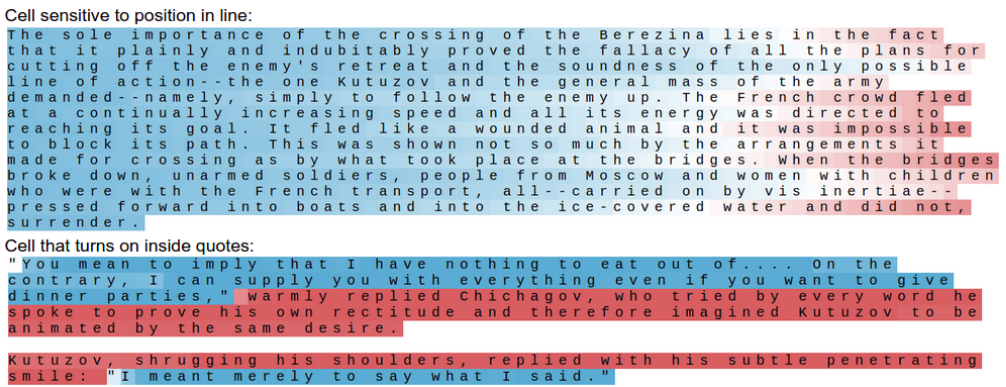
\includegraphics[width=\textwidth]{images/karpathy}
%
%\url{http://karpathy.github.io/2015/05/21/rnn-effectiveness/}
%\end{frame}


\input{images/activations.tikz}
\begin{frame}
\frametitle{Internal States Encode increasingly Classification Features}
\framesubtitle{LSTM cell \textbf{47} of 256}
\figactivations{1}{3}
\end{frame}
%%
%
\begin{frame}
\frametitle{Found Cloud Masking Cells in the RNN}
\framesubtitle{LSTM cell \textbf{47} of 256}
\figactivations{1}{47}
\end{frame}

\begin{frame}
\frametitle{Gate Activations are complicated}

\begin{itemize}
\item something seems to happen with the gates given the input
\item hard to visually interpret
\item still classification accuracy circa 80\% $\leftarrow$ gates seem to follow a purpose
\item information likely encoded in a linear combination in multiple dimensions over multiple layers
\item the designed purpose of the gates \emph{input},\emph{forget},\emph{output}, etc. may not be very meaningful
\end{itemize}
\end{frame}

{\setbeamercolor{background canvas}{bg=tumbluedark}
\begin{frame}[plain]

\vspace{8em}
\begin{center}
\Huge\color{tumwhite}
Let's do a input feature importance analysis
\end{center}\color{white}

\end{frame}
}

{\setbeamercolor{background canvas}{bg=white}
\begin{frame}[plain]

\vspace{8em}
\begin{center}
\Huge\color{tumbluedark}
with \textbf{gradients}
\end{center}\color{white}

\end{frame}
}

\begin{frame}
\only<1-3>{\frametitle{Usually we use gradients to adjust $\Mweight$...}}
\only<4->{\frametitle{We can also backprop to $\M{X}$}}

\begin{tikzpicture}
\node[font=\Huge](grad){
\only<1-3>{
$\frac{\partial \mathcal{L}(\V{y},f_\Mweight(\M{X}))}{\partial \Mweight}$
}
\only<4->{
$\frac{\partial \max(\yhat)}{\partial \M{X}}$
}
};

\node[above left=of grad, text width=12em](annotdx){
\only<2,3>{how do we have to change the network weights $\Mweight$...}
\only<4,5>{what changes in the input $\M{X}$...} 
};
\node[below right=of grad, text width=12em](annotdy){
\only<3>{... to change (minimize) the loss $\mathcal{L}$?}
\only<5>{... would change the predicted score $\max(\yhat) = \max(\f_\Mweight(\VInput))$?}
};

\visible<2,3,4,5>{\draw[-stealth, shorten >= 1em, rounded corners] (annotdx) -| ($ (annotdx)!0.5!(grad) $) |- ($ (grad)+(-.5em, -1em) $);}
\visible<3,5>{\draw[-stealth, shorten >= 1em, rounded corners] (annotdy) -| ($ (annotdy)!0.5!(grad) $) |- ($ (grad)+(2.5em, 1em) $);}

\end{tikzpicture}
\end{frame}

\begin{frame}
	\frametitle{Can be implemented in four lines}
	
		
	\Large $\frac{\partial \max(\yhat)}{\partial \M{X}}$ implementation
	
	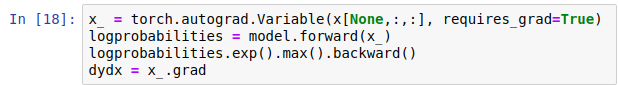
\includegraphics[width=\textwidth]{images/dydx_code}
	
	
\end{frame}


\begin{frame}
\begin{tikzpicture}

\frametitle{Gradients from $\max(\yhat)$ to \M{X}}
\framesubtitle{Example 1}


\def\root{images/rnn_examples/5}


\begin{groupplot}[
group style = {
group size = 1 by 3,
xlabels at=edge bottom,
xticklabels at=edge bottom,
vertical sep=0pt,
},
width=\textwidth,
%		hide axis,
enlargelimits=.1,
height=4cm,
%ymin=-.2, ymax=.2,
%no marks,
]
\nextgroupplot[draw opacity=.8, smooth=0.01, ylabel=$\M{X}$]
\addplot[b11color, mark=*,mark size=.5pt] table [x=t, y=B11, col sep=comma, forget plot] {\root/x.csv};
\addplot[b12color, mark=*,mark size=.5pt] table [x=t, y=B12, col sep=comma] {\root/x.csv};

\addplot[b5color, mark=*,mark size=.5pt] table [x=t, y=B5, col sep=comma, forget plot] {\root/x.csv};
\addplot[b6color, mark=*,mark size=.5pt] table [x=t, y=B6, col sep=comma, forget plot] {\root/x.csv};
\addplot[b7color, mark=*,mark size=.5pt] table [x=t, y=B7, col sep=comma, forget plot] {\root/x.csv};
\addplot[b8color, mark=*,mark size=.5pt] table [x=t, y=B8, col sep=comma, forget plot] {\root/x.csv};
\addplot[b8Acolor, mark=*,mark size=.5pt] table [x=t, y=B8A, col sep=comma] {\root/x.csv};

\addplot[b2color, mark=*,mark size=.5pt] table [x=t, y=B2, col sep=comma, forget plot] {\root/x.csv};
\addplot[b3color, mark=*,mark size=.5pt] table [x=t, y=B3, col sep=comma, forget plot] {\root/x.csv};
\addplot[b4color, mark=*,mark size=.5pt] table [x=t, y=B4, col sep=comma] {\root/x.csv};

\nextgroupplot[draw opacity=.8, smooth=0.01, ylabel=$\frac{\partial \max(\yhat)}{\partial \V{X}}$]
\addplot[b11color, mark=*,mark size=.5pt] table [x=t, y=B11, col sep=comma, forget plot] {\root/dydx.csv};
\addplot[b12color, mark=*,mark size=.5pt] table [x=t, y=B12, col sep=comma] {\root/dydx.csv};

\addplot[b5color, mark=*,mark size=.5pt] table [x=t, y=B5, col sep=comma, forget plot] {\root/dydx.csv};
\addplot[b6color, mark=*,mark size=.5pt] table [x=t, y=B6, col sep=comma, forget plot] {\root/dydx.csv};
\addplot[b7color, mark=*,mark size=.5pt] table [x=t, y=B7, col sep=comma, forget plot] {\root/dydx.csv};
\addplot[b8color, mark=*,mark size=.5pt] table [x=t, y=B8, col sep=comma, forget plot] {\root/dydx.csv};
\addplot[b8Acolor, mark=*,mark size=.5pt] table [x=t, y=B8A, col sep=comma] {\root/dydx.csv};

\addplot[b2color, mark=*,mark size=.5pt] table [x=t, y=B2, col sep=comma, forget plot] {\root/dydx.csv};
\addplot[b3color, mark=*,mark size=.5pt] table [x=t, y=B3, col sep=comma, forget plot] {\root/dydx.csv};
\addplot[b4color, mark=*,mark size=.5pt] table [x=t, y=B4, col sep=comma] {\root/dydx.csv};

\end{groupplot}
\end{tikzpicture}
\end{frame}


\begin{frame}
\begin{tikzpicture}

\frametitle{Gradients from $\max(\yhat)$ to \M{X}}
\framesubtitle{Example 2}

\def\root{images/rnn_examples/6}


\begin{groupplot}[
group style = {
group size = 1 by 3,
xlabels at=edge bottom,
xticklabels at=edge bottom,
vertical sep=0pt,
},
width=\textwidth,
%		hide axis,
enlargelimits=.1,
height=4cm,
%ymin=-.2, ymax=.2,
%no marks,
]
\nextgroupplot[draw opacity=.8, smooth=0.01, ylabel=$\M{X}$]
\addplot[b11color, mark=*,mark size=.5pt] table [x=t, y=B11, col sep=comma, forget plot] {\root/x.csv};
\addplot[b12color, mark=*,mark size=.5pt] table [x=t, y=B12, col sep=comma] {\root/x.csv};

\addplot[b5color, mark=*,mark size=.5pt] table [x=t, y=B5, col sep=comma, forget plot] {\root/x.csv};
\addplot[b6color, mark=*,mark size=.5pt] table [x=t, y=B6, col sep=comma, forget plot] {\root/x.csv};
\addplot[b7color, mark=*,mark size=.5pt] table [x=t, y=B7, col sep=comma, forget plot] {\root/x.csv};
\addplot[b8color, mark=*,mark size=.5pt] table [x=t, y=B8, col sep=comma, forget plot] {\root/x.csv};
\addplot[b8Acolor, mark=*,mark size=.5pt] table [x=t, y=B8A, col sep=comma] {\root/x.csv};

\addplot[b2color, mark=*,mark size=.5pt] table [x=t, y=B2, col sep=comma, forget plot] {\root/x.csv};
\addplot[b3color, mark=*,mark size=.5pt] table [x=t, y=B3, col sep=comma, forget plot] {\root/x.csv};
\addplot[b4color, mark=*,mark size=.5pt] table [x=t, y=B4, col sep=comma] {\root/x.csv};

\nextgroupplot[draw opacity=.8, smooth=0.01, ylabel=$\frac{\partial \max(\yhat)}{\partial \V{X}}$]
\addplot[b11color, mark=*,mark size=.5pt] table [x=t, y=B11, col sep=comma, forget plot] {\root/dydx.csv};
\addplot[b12color, mark=*,mark size=.5pt] table [x=t, y=B12, col sep=comma] {\root/dydx.csv};

\addplot[b5color, mark=*,mark size=.5pt] table [x=t, y=B5, col sep=comma, forget plot] {\root/dydx.csv};
\addplot[b6color, mark=*,mark size=.5pt] table [x=t, y=B6, col sep=comma, forget plot] {\root/dydx.csv};
\addplot[b7color, mark=*,mark size=.5pt] table [x=t, y=B7, col sep=comma, forget plot] {\root/dydx.csv};
\addplot[b8color, mark=*,mark size=.5pt] table [x=t, y=B8, col sep=comma, forget plot] {\root/dydx.csv};
\addplot[b8Acolor, mark=*,mark size=.5pt] table [x=t, y=B8A, col sep=comma] {\root/dydx.csv};

\addplot[b2color, mark=*,mark size=.5pt] table [x=t, y=B2, col sep=comma, forget plot] {\root/dydx.csv};
\addplot[b3color, mark=*,mark size=.5pt] table [x=t, y=B3, col sep=comma, forget plot] {\root/dydx.csv};
\addplot[b4color, mark=*,mark size=.5pt] table [x=t, y=B4, col sep=comma] {\root/dydx.csv};

\end{groupplot}
\end{tikzpicture}
\end{frame}


\begin{frame}
\begin{tikzpicture}

\frametitle{Gradients from $\max(\yhat)$ to \M{X}}
\framesubtitle{Example 3}

\def\root{images/rnn_examples/7}


\begin{groupplot}[
group style = {
group size = 1 by 3,
xlabels at=edge bottom,
xticklabels at=edge bottom,
vertical sep=0pt,
},
width=\textwidth,
%		hide axis,
enlargelimits=.1,
height=4cm,
%ymin=-.2, ymax=.2,
%no marks,
]
\nextgroupplot[draw opacity=.8, smooth=0.01, ylabel=$\M{X}$]
\addplot[b11color, mark=*,mark size=.5pt] table [x=t, y=B11, col sep=comma, forget plot] {\root/x.csv};
\addplot[b12color, mark=*,mark size=.5pt] table [x=t, y=B12, col sep=comma] {\root/x.csv};

\addplot[b5color, mark=*,mark size=.5pt] table [x=t, y=B5, col sep=comma, forget plot] {\root/x.csv};
\addplot[b6color, mark=*,mark size=.5pt] table [x=t, y=B6, col sep=comma, forget plot] {\root/x.csv};
\addplot[b7color, mark=*,mark size=.5pt] table [x=t, y=B7, col sep=comma, forget plot] {\root/x.csv};
\addplot[b8color, mark=*,mark size=.5pt] table [x=t, y=B8, col sep=comma, forget plot] {\root/x.csv};
\addplot[b8Acolor, mark=*,mark size=.5pt] table [x=t, y=B8A, col sep=comma] {\root/x.csv};

\addplot[b2color, mark=*,mark size=.5pt] table [x=t, y=B2, col sep=comma, forget plot] {\root/x.csv};
\addplot[b3color, mark=*,mark size=.5pt] table [x=t, y=B3, col sep=comma, forget plot] {\root/x.csv};
\addplot[b4color, mark=*,mark size=.5pt] table [x=t, y=B4, col sep=comma] {\root/x.csv};

\nextgroupplot[draw opacity=.8, smooth=0.01, ylabel=$\frac{\partial \max(\yhat)}{\partial \V{X}}$]
\addplot[b11color, mark=*,mark size=.5pt] table [x=t, y=B11, col sep=comma, forget plot] {\root/dydx.csv};
\addplot[b12color, mark=*,mark size=.5pt] table [x=t, y=B12, col sep=comma] {\root/dydx.csv};

\addplot[b5color, mark=*,mark size=.5pt] table [x=t, y=B5, col sep=comma, forget plot] {\root/dydx.csv};
\addplot[b6color, mark=*,mark size=.5pt] table [x=t, y=B6, col sep=comma, forget plot] {\root/dydx.csv};
\addplot[b7color, mark=*,mark size=.5pt] table [x=t, y=B7, col sep=comma, forget plot] {\root/dydx.csv};
\addplot[b8color, mark=*,mark size=.5pt] table [x=t, y=B8, col sep=comma, forget plot] {\root/dydx.csv};
\addplot[b8Acolor, mark=*,mark size=.5pt] table [x=t, y=B8A, col sep=comma] {\root/dydx.csv};

\addplot[b2color, mark=*,mark size=.5pt] table [x=t, y=B2, col sep=comma, forget plot] {\root/dydx.csv};
\addplot[b3color, mark=*,mark size=.5pt] table [x=t, y=B3, col sep=comma, forget plot] {\root/dydx.csv};
\addplot[b4color, mark=*,mark size=.5pt] table [x=t, y=B4, col sep=comma] {\root/dydx.csv};

\end{groupplot}
\end{tikzpicture}
\end{frame}

\begin{frame}
	\frametitle{Jupyter Notebook}
	
	
	\Large
	\textbf{github.com/marccoru/phiweek19/recurrence.ipynb}
		
\end{frame}
%
%\def\fps{3}
%\input{images/cells.tikz}
%
%\begin{frame}[t]
%\frametitle{Extracting features from noisy data with ConvRNNs}
%
%\centering
%%\lstmanim
%\begin{tikzpicture}[scale=1, node distance=2em]%,show background rectangle,background rectangle/.style={draw=red}]
%
%
%\draw pic (LSTM) at (0,0) {lstmanim};
%\node[io,xshift=1ex,above=3em of LSTMtl, ,label=above:$\VInput_{t}$](xt){\animategraphics[poster=25,width=1cm,autoplay,loop]{\fps}{images/activations/16494/x/x-}{1}{36}};%$x_{t}$
%\draw[rounded corners] (xt) |- (LSTM-input);
%\node[io,left=of LSTMtl,label=below:$\VHidden_{t-1}$](htminus1){
%	\animategraphics[poster=24,width=1cm,autoplay,loop]{\fps}{images/activations/16494/output/3-}{0}{35}
%};
%\draw[endflow] (htminus1) -- (LSTM-input);
%\node[io,right=of LSTMbr,label=above:$\VCellState_{t}$](ct){\animategraphics[poster=25,width=1cm,autoplay,loop]{\fps}{images/activations/16494/state/3-}{1}{36}}; % $c_{t}$
%\draw[endflow] (LSTM-coutput)--(ct);
%\node[io,left=of LSTMbl,label=above:$\VCellState_{t-1}$](ctminus1){\animategraphics[poster=24,width=1cm,autoplay,loop]{\fps}{images/activations/16494/state/3-}{0}{35}}; % 
%\draw[endflow] (ctminus1)--(LSTMfmult);
%\node[io,right=of LSTMtr,label=below:$\VHidden_{t}$](ht){
%	\animategraphics[poster=24,width=1cm,autoplay,loop]{\fps}{images/activations/16494/output/3-}{1}{36}
%%};
%\draw[endflow] (LSTM-houtput)--(ht);
%
%\draw[endflow] (ct) -- ($ (ct)+(0,-0.8) $) -| (ctminus1);
%\draw[endflow] (ht) -- ($ (ht)+(0,.8) $) -| (htminus1);
%
%\end{tikzpicture}
%
%\end{frame}